% requirements:
%	TeX environments: TeXlive/MacTeX or MiKTeX
%	compiler: XeLaTeX
%
% ---------------------------------------------------------------------------- %
%                                   preamble                                   %
% ---------------------------------------------------------------------------- %
\documentclass[a4paper]{article}
% 10.5pt = 5 hao

% ---------------------------------- layout ---------------------------------- %
\usepackage[a4paper,top=2.5cm,bottom=2.5cm,left=3cm,right=3cm,% margins
			headheight=1.5cm,headsep=1.5em,
			footskip=2em,
			]{geometry}

% ------------------------------- math symbols ------------------------------- %
% 载入常用的数学包, 符号包
\usepackage{amsmath}
\usepackage{amsfonts}
\usepackage{amssymb}
\usepackage{mathrsfs}
\usepackage{blindtext}
\usepackage{minted}

%----------------------------------------------------------------%
%% linespace 行间距,段间距等等
\usepackage{setspace}
% \usepackage{indentfirst} % then the first line of each title should start with a indent.
% 定义标题和段落样式
% 定义1.5倍行距
\renewcommand{\baselinestretch}{1.62}
\setlength{\baselineskip}{12pt}   % set the fixed value of the lineskip
\setlength\parskip{\baselineskip} % set the space between the paragraphs, set the variable \parskip \baselineskip
% parindent
\setlength{\parindent}{0pt}

%----------------------------------------------------------------%
% fonts (style, color, size). 字体的大小,颜色,以及定义常用的字号
\usepackage{ctex}		 	% If you are lazy, the CTEX suit is enough.
% Chinese font
\usepackage{xeCJK}		 	% For the Chinese through XeLaTex
\setCJKmainfont{SimSun} 	% set the mainfont of Chinese as songti. (serif) for
\setCJKsansfont{SimSun} 	% sans serif font for \textsf
\setCJKmonofont{SimSun} 	% monospace font for \texttt
% \punctstyle{kaiming}  	% Remove the space used by symbols like comma. Special for the mainland students like us HUSTers.
\setCJKfamilyfont{song}{SimSun}                       % 宋体 song
\newcommand{\song}{\CJKfamily{song}}
\setCJKfamilyfont{kai}{KaiTi}                         % 楷体  kai
\newcommand{\kai}{\CJKfamily{kai}}
\setCJKfamilyfont{hwzs}{STZhongsong}                  % 华文中宋  hwzs
\newcommand{\hwzs}{\CJKfamily{hwzs}}
\setCJKfamilyfont{hei}{SimHei}                        % 黑体  hei
\newcommand{\hei}{\CJKfamily{hei}}
% English font
\usepackage{fontspec}% Then you can use the fonts installed at your device.
\setmainfont{Times New Roman}
\setsansfont{Times New Roman}
\setmonofont{Times New Roman}
%\setsansfont{[foo.ttf]} % for the fonts at this default path.
% font Color 利用definecolor自己可以定义颜色
\usepackage{xcolor}
\definecolor{MSBlue}{rgb}{.204,.353,.541}
\definecolor{MSLightBlue}{rgb}{.31,.506,.741}
% font Size (I use pinyin represents the corresponding size in Microsorft Word)
% \newcommand{\chuhao}{\fontsize{42pt}{\baselineskip}\selectfont}
\newcommand{\xiaochuhao}{\fontsize{36pt}{\baselineskip}\selectfont}
% \newcommand{\yihao}{\fontsize{28pt}{\baselineskip}\selectfont}
\newcommand{\erhao}{\fontsize{21pt}{\baselineskip}\selectfont}
\newcommand{\xiaoerhao}{\fontsize{18pt}{\baselineskip}\selectfont}
\newcommand{\sanhao}{\fontsize{15.75pt}{\baselineskip}\selectfont}
\newcommand{\sihao}{\fontsize{14pt}{18pt}\selectfont}
\newcommand{\xiaosihao}{\fontsize{12pt}{18pt}\selectfont}
\newcommand{\wuhao}{\fontsize{10.5pt}{18pt}\selectfont}
% \newcommand{\xiaowuhao}{\fontsize{9pt}{\baselineskip}\selectfont}
% \newcommand{\liuhao}{\fontsize{7.875pt}{\baselineskip}\selectfont}
% \newcommand{\qihao}{\fontsize{5.25pt}{\baselineskip}\selectfont}


% ---------------------------------------------------------------------------- %
%% header and footer 页眉,页脚
\usepackage{fancyhdr} % for header and footer

% 设置页眉样式
\newcommand{\headstyle}{
 \fancyhead[C]{ \hwzs\wuhao 华\hspace{0.5em}中\hspace{0.5em}科\hspace{0.5em}技\hspace{0.5em}大\hspace{0.5em}学\hspace{0.5em}课\hspace{0.5em}程\hspace{0.5em}设\hspace{0.5em}计\hspace{0.5em}(报\hspace{0.5em}告)}
}

% 设置页脚样式
\newcommand{\footstyle}{\fancyfoot[C]{\wuhao\thepage}
 \fancyfoot[L]{\rule[5pt]{6.7cm}{0.4pt}}
 \fancyfoot[R]{\rule[5pt]{6.7cm}{0.4pt}}
}
\pagestyle{fancy}
\fancyhf{} % 清空原有样式
\headstyle
\footstyle
% 定义一种新的格式叫做main
\fancypagestyle{main}{%
 \fancyhf{} % 清空原有样式
 \headstyle
 \footstyle
}
\renewcommand{\headrulewidth}{0.4pt}
% \renewcommand{\footrulewidth}{0.4pt}
% \renewcommand{\headrule}{\rule{\textwidth}{0.4pt}}

% ---------------------------------------------------------------------------- %
% set the styles of sections at all levels
% 设置各个标题样式
% 不需要使用part和chapter层级
\usepackage{titlesec}
\usepackage{titletoc}
\titleformat{\section}{\centering\hei\bfseries\xiaoerhao}{\thesection}{1em}{} % 在section标题编号后面加个点
% \titlelabel{\thetitle.\quad} % add a dot after the counter for all levels of sections
% \titleformat*{\section}{\wuhao\bfseries} % 设置标签的形式,5号加粗
\titleformat*{\subsection}{\raggedright\hei\bfseries\sihao}
\titleformat*{\subsubsection}{\raggedright\hei\bfseries\xiaosihao}
\titleformat{\paragraph}[hang]{\raggedright\hei\bfseries\xiaosihao}{\theparagraph}{1em}{}[]

% manual
% \titleformat{command}[shape]{format}{label}{sep}{before-code}[after-code]
% \titlespacing{command}{left}{before-sep}{after-sep}
% 设置新的层级subsubsubsection
\setcounter{tocdepth}{4}
\setcounter{secnumdepth}{4}

\newcommand{\sectionbreak}{\clearpage} % 小节从新的一页开始
% 根据学校要求设置新的section, subsection, subsection,  paragraph

% set the content of section and so on
\newcommand\seccontent{
	\song
	\xiaosihao % 默认五号字体, 行间距为1.5*\baselineskip
    \setlength{\parindent}{2em} % 首段缩进两个M字符
    \setlength{\parskip}{0pt}
    }
\newcommand\tabcontent{
	\song
	\wuhao % 默认五号字体, 行间距为1.5*\baselineskip
	\setlength{\parindent}{2em} % 首段缩进两个M字符
	\setlength{\parskip}{0pt}
}


% ---------------------------------------------------------------------------- %
% for the style of theorems, definitions, proofs and remarks 定义数学里面一些常用的环境
\usepackage{amsthm}
\newtheorem{thm}{\textbf{定理}}[section]
% The section in [] can be replaced by chapter or subsection
\theoremstyle{definition} 
\theoremstyle{plain}
\theoremstyle{remark}

% ---------------------------------------------------------------------------- %
% for the caption and reference 图表及公式的编号规范
\usepackage{float} 		 		  	% table figure positioning
\usepackage{caption}
\captionsetup[figure]{labelformat=default, labelsep=quad,name={图}}
\captionsetup[table]{labelformat=default,labelsep=quad,name={表}}
% 设置图表标题的计数方式
\renewcommand{\thefigure}{\ifnum \thesection>0 \thesection-\fi \arabic{figure}} % set caption label style to 2-1
\renewcommand{\thetable}{\ifnum \thesection>0 \thesection-\fi \arabic{table}} % set caption label style to 2-1
\DeclareCaptionFont{mylabelfont}{\hei\xiaosihao}
\captionsetup[figure]{font=mylabelfont}
\captionsetup[table]{font=mylabelfont}

% 设置图表的autoref的格式
\newcommand{\reffig}[1]{图 \ref{#1}}
\newcommand{\reftab}[1]{表 \ref{#1}}
% 公式的编号格式
\renewcommand\theequation{\arabic{section}-\arabic{equation}}

\usepackage{graphicx} % To include graphixs 添加图所需的包

\graphicspath{{./graphics/}} %设置图片路径
\usepackage{booktabs} % To create three line table including the commands toprule, bottomrule, and midrule
% \usepackage{colortbl} %
% 使用tabularx库并定义新的左右中格式
\usepackage{tabularx}
\usepackage{makecell}
\newcolumntype{L}{X}
\newcolumntype{C}{>{\centering \arraybackslash}X}
\newcolumntype{R}{>{\raggedright \arraybackslash}X}

% ---------------------------------------------------------------------------- %
% set the style of counters 设置计数器
% 设置重新计数的位置
\makeatletter
\@addtoreset{footnote}{page}
\@addtoreset{figure}{section}
\@addtoreset{table}{section}
\@addtoreset{equation}{section}
\makeatother

% ---------------------------------------------------------------------------- %
% tableofcontents, listoftables and listoffigures 目录
%\renewcommand\listfigurename{插图列表}
%\renewcommand\listtablename{表格列表}
%\titlecontents{标题名}[左间距]{标题格式}{标题标志}{无序号标题}{指引线与页码}[下间距]
%\dottedcontents{section}[2.55em]{\song \xiaosihao \bfseries}{2.5em}{1em}
\usepackage{tocloft}
\renewcommand{\contentsname}{\centerline{ \hei\bfseries\xiaoerhao 目\hspace{2em}录}}
\titlecontents{section}[3em]{\song\xiaosihao\bfseries}{\contentslabel{3em}}{\hspace*{-3em}}{\normalfont\titlerule*[8pt]{.}\contentspage}
\titlecontents{subsection}[3em]{\song\xiaosihao}{\contentslabel{3em}}{\hspace*{-3em}}{\titlerule*[8pt]{.}\contentspage}
\titlecontents{subsubsection}[4em]{\song\xiaosihao}{\contentslabel{4em}}{\hspace*{-4em}}{\titlerule*[8pt]{.}\contentspage}
\titlecontents{paragraph}[5em]{\song\xiaosihao}{\contentslabel{5em}}{\hspace*{-5em}}{\titlerule*[8pt]{.}\contentspage}

% ---------------------------------------------------------------------------- %
% reference and citation 参考文献
\usepackage{natbib}
\renewcommand{\refname}{\centering\hei\xiaoerhao 参考文献}
\bibsep=0pt % 用来设置每个\bibitem之间的间距
% \renewcommand{\bibname}{HUSTthesis} % .bib name
% \newcommand{\upcite}[1]{\textsuperscript{\textsuperscript{\cite{#1}}}} % show citation label in the upperscript

% ---------------------------------------------------------------------------- %
% 设置声明页
% 使用特殊符号
\usepackage{amssymb}
\usepackage{wasysym}
% 制作tatement中的符号
\def\HUSTcheckedbox{$\Square\!\!\!\!\checkmark$}
\def\HUSTbox{$\Square$}


% ---------------------------------------------------------------------------- %
% 定义中英文摘要和致谢环境
%
% 中文摘要环境
\newenvironment{cnabstract}[1]{
	\def \cnkeyword {#1}
	\clearpage
	\phantomsection
	\addcontentsline{toc}{section}{摘要}
	\vspace*{-20pt}
	\begin{center}
		\heiti \bfseries \xiaoerhao 摘 \hspace{2em} 要
	\end{center}
	\seccontent
}{
	\vspace{1em}
	\par\noindent {\hei\sihao \bfseries 关键词:} {\song\xiaosihao\cnkeyword}

}

% 英文摘要环境
\newenvironment{enabstract}[1]{
	\def \enkeyword {#1}
	\clearpage
	\phantomsection
	\addcontentsline{toc}{section}{Abstract}
	\vspace*{-20pt}
	\begin{center}
		\bfseries \xiaoerhao Abstract
	\end{center}
	\seccontent
}{
	\vspace{1em}
	\par\noindent {\sihao\bfseries Key Words: }\ {\song\xiaosihao\enkeyword}
	\clearpage
}

% 定义致谢环境
\newenvironment{thankpage}{
	\clearpage%
	\phantomsection%
	\addcontentsline{toc}{section}{致谢}%
	\section*{致\hspace{2em}谢}%
}{
	\clearpage
}


% ---------------------------------------------------------------------------- %
%	---	定义列表项,列举的样式
\usepackage{enumitem}
\setlist{noitemsep}

% ---------------------------------------------------------------------------- %
% \usepackage{makeindex} For the index 索引
\usepackage{listings} % For the code. 代码

% ---------------------------------------------------------------------------- %
% 设置脚注

% ---------------------------------------------------------------------------- %
%% For the hyperlink and bookmark 超链接及书签,(这样生成的pdf中的引用直接点击链接即可到达目的地)
\usepackage[bookmarks=true,colorlinks,linkcolor=black,citecolor=black,urlcolor=purple]{hyperref}% 设置超链接并修改风格


% ---------------------------------------------------------------------------- %
%% For the appendix, 附录
% 设置附录
\usepackage{appendix}
\renewcommand{\appendixname}{附录}

% ---------------------------------------------------------------------------- %
% for the titlepage 标题页,此处可以省略,建议直接使用官方给出的标题页即可
\usepackage{titling}
% 重置命令 maketitle
\renewcommand{\maketitle}{
	\def\HUSTtitlelength{12em}
 	\begin{titlepage}
		\begin{center}
			\vspace*{0em}
			\includegraphics[height=1.61cm]{HUSTlogo.eps}\\
%
			\vspace*{4em}
%
			{\xiaochuhao \hwzs \bfseries 单片机课程结课设计}\\
%
			\vspace*{6em}
			{\erhao \hei \bfseries \thetitle}

			\vspace*{6em}
			{\sanhao \hwzs
				\renewcommand\arraystretch{2.7}
				\begin{tabular}{lc}
					\makebox[4em][s]{院 \hfill 系} &
					\underline{\makebox[\HUSTtitlelength]{\school}} \\
					\makebox[4em][s]{专业班级} &
					\underline{\makebox[\HUSTtitlelength]{\classnum}} \\
					\makebox[4em][s]{姓 \hfill 名} &
					\underline{\makebox[\HUSTtitlelength]{\theauthor}} \\
					\makebox[4em][s]{学 \hfill 号} &
					\underline{\makebox[\HUSTtitlelength]{\stunum}} \\
					\makebox[4em][s]{指导教师} &
					\underline{\makebox[\HUSTtitlelength]{\instructor}} \\
			  \end{tabular}
		    }

			\vspace{4em}
			{\sanhao \hwzs \thedate}

		\end{center}
	\end{titlepage}
}

% ------------------------------------ 标题页 ----------------------------------- %
\title{简易数控直流电源设计} % 论文题目
\def\school{电子信息与通信学院} % 院系
\def\classnum{信卓2201班} % 专业班级
\author{董浩} % 姓名
\def\stunum{U202213781}	% 学号
\def\instructor{肖波} % 指导老师
\date{\today} % 日期

% -------------------------------- quickinput -------------------------------- %
% 利用\newcommand{cmd}{def} 设置一些常用的代码,提高效率,这里可以自行删除,下面是我敲翻译时候打的一些command。
\newcommand{\hongzifuzhu}[1]{\textcolor{red}{\kai \wuhao(#1)}}

% ---------------------------------------------------------------------------- %
%                                   document                                   %
% ---------------------------------------------------------------------------- %
\begin{document}

\maketitle % 生成标题页,个人建议直接使用学校给的word转成pdf与这里生成的pdf第一页合并,再去打印封皮。

% \thispagestyle{empty}% 标题页不参与编号
% ------------------------------------ 声明页 ----------------------------------- %
\setcounter{page}{1}
\renewcommand{\thepage}{\Roman{page}}


% ----------------------------------- 中文摘要 ----------------------------------- %
\setcounter{page}{1}
\renewcommand{\thepage}{\Roman{page}}
\begin{cnabstract}{可调电源; 串口调节; STM32F407ZGT6; LM117; LM358}
	\hspace{2em}
	本设计制作的可调节数控电源系统,可以输出稳定的电压,通过按键进行精度为0.1V的调节,并在LCD1602屏幕和串口上显示当前电压值和电压设置值。系统由 LCD1602、LM117、 ADC(开发板内置)、DAC(开发板内置)、和STM32F407ZGT6开发板等部分组成。DAC输出按键设置的电压,通过LM117电压调节电路输出电压,ADC采集电压信息,将信息通过串口和LCD1602输出,同时进行PID调节稳定电压。
\end{cnabstract}

\newpage

\tableofcontents
\thispagestyle{main}


\clearpage
\setcounter{page}{1}
\renewcommand{\thepage}{\arabic{page}}

% ----------------------------------- 主体内容 ----------------------------------- %
\seccontent
\section{设计要求}

\subsection{具体要求}
\begin{itemize}
	\item 可使用按键设置电压;
	\item PC机可通过串口向数控电源发送指令,设置电压;
	\item 数控电源通过串口每2秒钟向发送1次当前电压值;
	\item 输出电压范围0至+9.9V,步进0.1V;
	\item 最大输出电流:200mA;
	\item 在1602液晶屏上显示当前电压值,以及电压设置值;
	\item 使用洞洞板焊接核心电路;
	\item 输出端预留一个电源座或接线柱以便挂接负载电阻。
	
\end{itemize}

\subsection{设计框图}
\vspace*{-2em}
\begin{figure}[H]
	\centering
	\includegraphics[width=1\textwidth]{设计框图}
	\caption{设计框图}
	\label{E8}
\end{figure}

\sectionbreak


\section{设计思路}

\subsection{系统框图}
\begin{figure}[H]
	\centering
	\includegraphics[width=1.1\textwidth]{实现框图}
	\caption{实现框图}
\end{figure}
\subsection{核心原理图}
\vspace*{-2em}
\begin{figure}[H]
	\centering
	\includegraphics[width=1\textwidth]{原理图}
	\caption{原理图}
\end{figure}

\subsection{方案描述}
\subsubsection{电路部分}
使用LM358运算放大器和LM317稳压器制作输出电压可变的稳压电源。LM358使用±12V直流恒压电源供电,LM317时钟+12V直流恒压电源供电,均设置限流0.50A。使用单片机DAC输出的电压作为控制电压,经过LM358和LM317处理后输出放大后的电压,为负载供电。电源、单片机和放大电路共地。

参数的选择方面,根据LM317的特性:
\begin{equation*}
	V_{OUT}=V_{REF}(1+\frac{R2}{R1}+I_{ADJ}R2)
\end{equation*}
以及$V_{OUT}$和$ADJ$之间1.25V的标准参考电压,结合LM358的工作原理,确定$R1=300\Omega,\ R2=100\Omega$,从而控制输出电压与输入电压的比值为4。
\subsubsection{单片机部分}
\paragraph*{设计思路}
\vspace*{-0.5em}
总体思路为使用按键和串口通信更改存储的设定值,将设定值输入PID模块,生成电压输出值。再经过DAC模块输出电压,传递给外部电路。同时ADC模块对输出电压进行采样,写入测量值存储模块,进而输入到PID模块,达到闭环调节的目的。通信方面,PC机与单片机之间使用UART串口通信,串口通信模块读取设定值和测量值,将结果发送给PC机,从而在PC机上显示。单片机通过接收PC机发送的电压调节指令,更改设定值,从而达到使用PC机设置电压的目的。
\vspace*{-0.5em}
\paragraph*{硬件资源分配}
\vspace*{-0.5em}
\noindent 本项目使用的硬件资源如下:
\vspace*{-0.5em}
\begin{itemize}
	\item systick:用于delay函数的延时
	\item KEY0、KEY1:用于调节电压值
	\item TIM3:用于串口定时输出的计时
	\item EXTI line8 and line9:用于配置按键外部中断
	\item ADC1\_CH5:用于采样电压
	\item DAC1:用于输出指定电压
	\item USART1:用于和PC机进行串口通信
\end{itemize}
使用到的外部IO如下:
\begin{itemize}
	\item PA4:DAC1的输出引脚
	\item PA5:ADC1\_CH5的输入引脚
	\item PA9:UART的TX引脚
	\item PA10:UART的RX引脚
	\item PB8:开发板上自带的KEY1
	\item PB9:开发板上自带的KEY0
	\item PD8:连接LCD显示屏的RS极
	\item PD9:连接LCD显示屏的RW极
	\item PD10:连接LCD显示屏的EN极
	\item PF0-10:LCD显示屏数据输入
\end{itemize}

\subsection{小组分工}
本设计由三人合作完成,小组分工如下:
\begin{itemize}
	\item 董浩:主程序框架、通信指令、ADC、DAC、按键控制、电路仿真、 系统组装、电路调试
	\item 董星星:显示屏模块代码、ADC采样部分、串口通信
	\item 雷雨田:PID算法代码,电路设计、洞洞板焊接、电路调试
\end{itemize}


\section{实现效果}
使用LTspice进行仿真,设置负载R为200$\Omega$,在直流扫描模式下,对Vin进行扫描,起始值0.1V,结束值3.3V,步进0.01V,收集测量值绘图如下:
\begin{figure}[H]
	\centering
	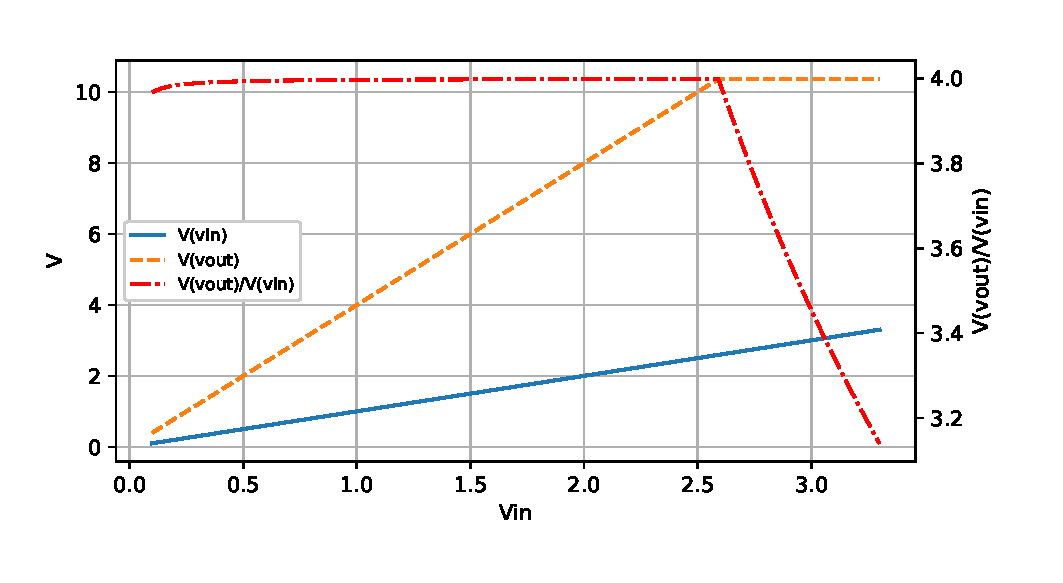
\includegraphics[width=1\textwidth]{仿真曲线}
	\caption{仿真曲线}
\end{figure}
由图可知,在200$\Omega$的负载下,输出最大电压可达到10V以上,且输入电压在0到2.5V的区间内时,输出电压与输入电压的比值为4,符合设计原理图时的预期。
完成仿真后,制作使用洞洞板制作原理图所示电路。洞洞板、LCD1602和单片机之间使用杜邦线相连,上电测试。系统工作正常,可以自由设定电压,输出指定电压,同时在LCD上显示设定电压和实际电压,并传输给PC主机,设计通过验收。
\sectionbreak

\section{不足与改进}
在实测中,发现电压调节不够迅速,带负载能力不够强以及电压存在mV级别的波动等问题,对有关问题进行分析,发现原因以及相应改进措施如下:

对于电压调节不够迅速,原程序在主函数的循环内不断调用LCD显示函数来刷新显示屏显示的数值,而显示函数中含有延时函数导致数据刷新和显示不及时。同时PID算法部分参数设置的值不够合理,导致电压变化过慢。针对这一问题,改进措施如下:使用定时器定时产生中断,产生中断时将标志位置1,主程序的循环中检测到该标志位后执行刷新LCD命令并将标志位置0,而从避免主程序不断刷新LCD导致电压调节不够迅速。

对于电压存在波动,采用在电路中添加滤波,去耦电容的方式,对输出进行整流,同时稳定电压。

针对带负载能力不够强,测试时发现对于12$\Omega$以下的电阻,输出电压的最大值在10V以下,暂未得出有效解决方案,考虑更换性能更好的运放或改进电路。对原电路,使用LTspice仿真导出数据后绘图如下:
\begin{figure}[H]
	\centering
	\includegraphics[width=1\textwidth]{电阻扫描}
	\caption{电阻扫描仿真曲线}
\end{figure}



\sectionbreak


% ------------------------------------ 附录 ------------------------------------ %
\clearpage
\appendix
\phantomsection
\addcontentsline{toc}{section}{附录}
\section*{附录}
本次实验验收时用到的原始代码如下:

中断服务函数部分:
\begin{minted}[breaklines]{C}
	// 配置按键中断服务函数
	void EXTI9_5_IRQHandler(void)
	{
		if (EXTI_GetITStatus(EXTI_Line9) != RESET) // KEY1按下
		{
			// LED0取反
			GPIO_ToggleBits(GPIOF, GPIO_Pin_9);
			target -= 100; // 设定值降低0.1V
			printf("使用按键设定值为%.3fV\r\n", target / 1000.0);
			EXTI_ClearITPendingBit(EXTI_Line9);
		}
		else if (EXTI_GetITStatus(EXTI_Line8) != RESET) // KEY0按下
		{
			// LED1取反
			GPIO_ToggleBits(GPIOF, GPIO_Pin_10);
			target += 100; // 设定值增加0.1V
			printf("使用按键设定值为%.3fV\r\n", target / 1000.0);
			EXTI_ClearITPendingBit(EXTI_Line8);
		}
	}
	// 定时器3中断服务函数
	// 每隔两秒输出一次值
	void TIM3_IRQHandler(void)
	{
		u16 adcx;
		if (TIM_GetITStatus(TIM3, TIM_IT_Update) == SET)
		{
			adcx = Get_Adc_Average(ADC_Channel_5, 20); // 获取通道5的转换值,20次取平均
			measure = (float)adcx * (3.3 / 4096);	   // 获取计算后的带小数的实际电压值,比如3.1111
			printf("AD采样电压为%.3fV\r\n", measure);
			printf("测量电压为%.3fV\r\n", 4 * measure);
			printf("采样完成\r\n");
		}
		TIM_ClearITPendingBit(TIM3, TIM_IT_Update); // 清除中断标志位
	}
\end{minted}
控制算法部分:
\begin{minted}[breaklines]{C}
	/*******pid.h*******/
	#ifndef _PID_H
	#define _PID_H
	
	typedef struct
	{
		double target_value;  // 设定的目标值及需要达到的最终值
		double current_value; // 当前值(可认为外部的反馈值)
		double CAL_value;     // 计算需要输出的值
		double sum_error;     // 累计的偏差值
		double error;         // 误差值
		double last_error;    // 上一次误差值
		double pre_error;     // 上上一次误差值(增量式pid中使用)
	} PID;
	
	double Velocity_FeedbackControl(double Targetvalue, double Currentvalue);
	extern PID pid;
	#endif
	
	/*******pid.c*******/
	#include "pid.h"
	#define Kp 0.10f
	#define Ki 0.25f
	#define Kd 0.00f
	
	PID pid;
	double output[100];
	
	double Velocity_FeedbackControl(double Targetvalue, double Currentvalue)
	{
		pid.last_error=pid.error;
		pid.error=Targetvalue-Currentvalue;
		pid.sum_error=pid.sum_error+(pid.error*Ki);
		pid.CAL_value=(pid.error-pid.last_error)*Kd+pid.error*Kp+pid.sum_error;
		return pid.CAL_value;
	}
\end{minted}
主程序部分:
\begin{minted}[breaklines]{C}
	#include "stm32f4xx.h"
	#include "delay.h"
	#include "LED.h"
	#include "key.h"
	#include "serial.h"
	#include "DAC.h"
	#include "time.h"
	#include "ADC.h"
	#include <string.h>
	#include "pid.h"
	#include "LCD.h"
	/*
	*****Attention***********
	****target使用4位整数****
	例:1234表示设定电压1.234V
	*************************
	*/
	float measure = 0; // 电压测量值
	u16 target = 1100; // 电压设定值
	char target_str[5];
	char measure_str[5];
	
	int main(void)
	{
		// 初始化部分
		Serial_Init(); // 波特率115200
		delay_init(168);
		LED_Init();							// 测试LED初始化
		Dac1_Init();						// DAC1输出初始化
		EXTI_Key_Config();					// 按键EXTI中断配置
		Adc_Init();							// ADC1_CH5初始化
		TIM3_Int_Init(20000 - 1, 8400 - 1); // TIM3初始化,每隔2秒自动中断
		LCD_Init();							// LED初始化
		LCD_Clear();						// 清屏
		pid.sum_error = 0;
		
		Dac1_Set_Vol(1100); // 设置DAC输出默认电压
		
		while (1)
		{
			if (Serial_GetRxFlag() == 1) // 接收到了数据
			{
				Serial_SendArray(Serial_RxPacket, 4);
				target = 1000 * Serial_RxPacket[0] + 100 * Serial_RxPacket[1] + 10 * Serial_RxPacket[2] + Serial_RxPacket[3]; // 目标值
				
				printf("使用串口设定值为%.3fV\r\n", target / 1000.0);
			}
			
			double tg = (double)target;
			Velocity_FeedbackControl(tg, pid.CAL_value);
			u16 tg_ = (u16)pid.CAL_value / 4.0;
			Dac1_Set_Vol(tg_); // 设置电压值为tg_
			
			sprintf(target_str, "%.3f", target / 1000.0);		                            	// 将target转换为字符串,存储到targrt_str中
			sprintf(measure_str, "%.3f", 4 * measure);	  // 将measure转换为字符串,存储到measure_str中
			LCD_Display_Str(1, 1, "Target  :");
			LCD_Display_Str(2, 1, "Measure :");
			
			LCD_Display_Str(1, 12, target_str);
			LCD_Display_Str(2, 12, measure_str);
		}
	}
\end{minted}
\end{document}
